%!TEX root = ../main.tex

\section{Implementation}

\note{NS: @João explain how the thing is currently implemented. Provide a few snapshots of the system.}


\section{Evaluation}

\note{NS: @João provide a list of the main results we want to add in here.}

\begin{figure}[t]
  \centering 
  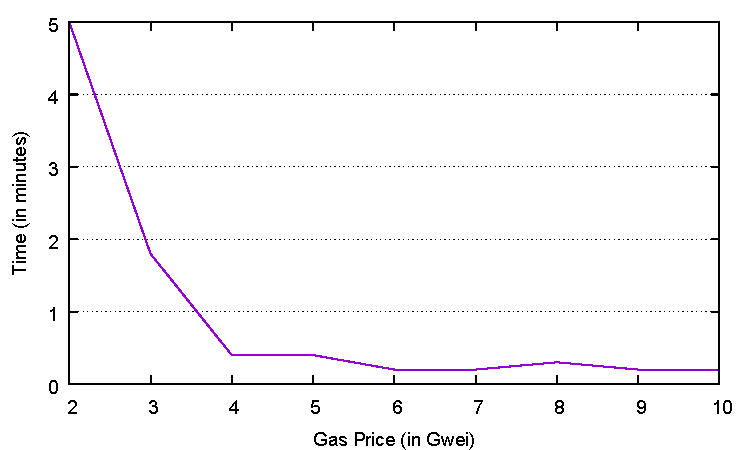
\includegraphics[width=\columnwidth]{final-figures/ethereum-confirmation-time.pdf}
  \vspace{-10pt}
  \caption{Ethereum transaction confirmation time in function of Gas Price.}
%  \vspace{-0.3cm}
  \label{fig:confirmationtime}
\end{figure}

\begin{table}[]
\centering
\begin{tabular}{@{}lll@{}}
\toprule
\textbf{\begin{tabular}[c]{@{}l@{}}Gas price \\ (Gwei)\end{tabular}} & \textbf{\begin{tabular}[c]{@{}l@{}}Contract Creation Cost \\ (in USD)\end{tabular}} & \textbf{\begin{tabular}[c]{@{}l@{}}Claim Issuance Cost\\  (in USD)\end{tabular}} \\ \midrule
\textbf{2}                                                           & 1,72                                                                                & 0,24                                                                             \\
\textbf{4}                                                           & 3,43                                                                                & 0,48                                                                             \\
\textbf{6}                                                           & 5,15                                                                                & 0,72                                                                             \\
\textbf{8}                                                           & 6,86                                                                                & 0,96                                                                             \\
\textbf{10}                                                          & 8,58                                                                                & 1,20                                                                             \\ \bottomrule
\end{tabular}
\caption{DClaims Ethereum Costs}
\label{my-label}
\end{table}



\begin{figure}[t]
  \centering
  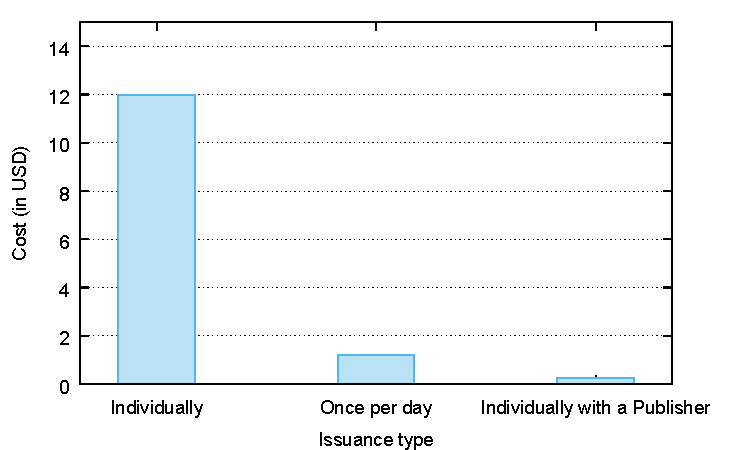
\includegraphics[width=\columnwidth]{final-figures/publisher-issuing-price.pdf}
  \vspace{-10pt}
  \caption{Cost of issuing claims in the different available ways.}
%  \vspace{-0.3cm}
  \label{fig:costpublishers}
\end{figure}

\begin{figure}[t]
  \centering
  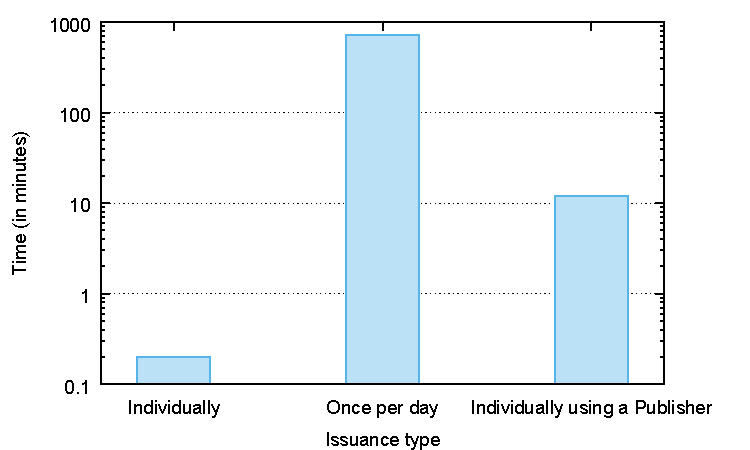
\includegraphics[width=\columnwidth]{final-figures/publisher-issuing-time.pdf}
  \vspace{-10pt}
  \caption{Time for claims to be confirmed on the Ethereum blockchain}
%  \vspace{-0.3cm}
  \label{fig:timepublishers}
\end{figure}

\begin{figure}[t]
  \centering
  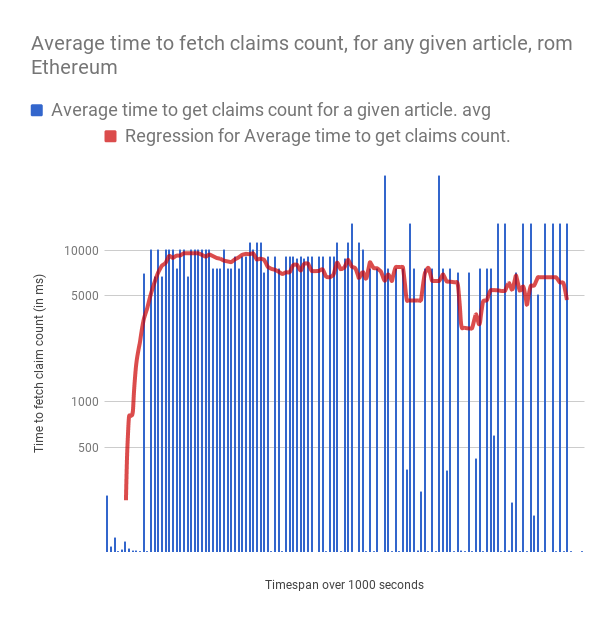
\includegraphics[width=\columnwidth]{mock-figures/ethereumfetch.png}
  \vspace{-10pt}
  \caption{Time to load a webpage as function of the number of articles. \note{NS: @João dont forget to add two curves: one with the other without DClaims.}}
%  \vspace{-0.3cm}
  \label{fig:ethereumfetch}
\end{figure}

\begin{figure}[t]
  \centering
  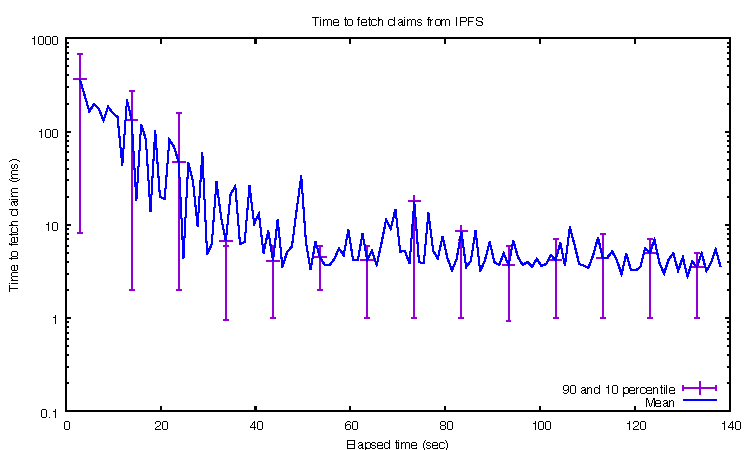
\includegraphics[width=\columnwidth]{mock-figures/ipfsfetch.pdf}
  \vspace{-10pt}
  \caption{Time to fetch individual claims from IPFS}
%  \vspace{-0.3cm}
  \label{fig:ipfsfetch}
\end{figure}

\subsection{Performance of Web Application}


In this section, we evaluate the impact of DClaims in terms of the user experience of the website. \note{NS: @João extend the same experiments for 5 sites, try to pick different sites.}

\begin{figure}[t]
  \centering
  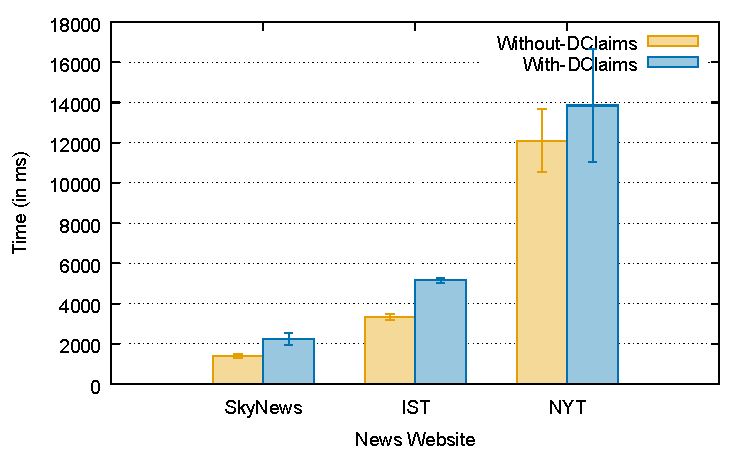
\includegraphics[width=\columnwidth]{final-figures/website-3-comparison.pdf}
  \vspace{-10pt}
  \caption{Loading time comparison of popular news websites with and without DClaims running.}
%  \vspace{-0.3cm}
  \label{fig:evalwebpage}
\end{figure}

\mypara{1. What's the overhead of loading a web page with DClaims?} Figure~\ref{fig:evalwebpage} shows the time it takes to fetch claims from three news websites, Instituto Superior Técnico, SkyNews and New York Times. We can see that the overhead introduced by DClaims is very low.

Figure \ref{fig:evalnarticles} is a benchmark test were we used a striped down version of a website as a basis and created several versions of that website, each with ten more news articles than the previous one. As the figure shows the overhead introduced by DClaims is proportional to the number of articles per page.

By comparing Figures \ref{fig:evalwebpage} and \ref{fig:evalnarticles} one might wonder why in the first, the overhead introduced by DClaims appears to be smaller than in the second. That happens because the website we used for the benchmark has been stripped down of any Javascript code, which slows down the loading time. The same does not happen in regular websites such as SkyNews and the New York Times. 

\note{JS: The conclusion here is that while when compared to super simplified websites, the overhead introduced by DClaims is significant, in the real world it is hardly noticed because regular websites are loaded with JS code that slows down the loading time}

\begin{figure}[t]
  \centering
  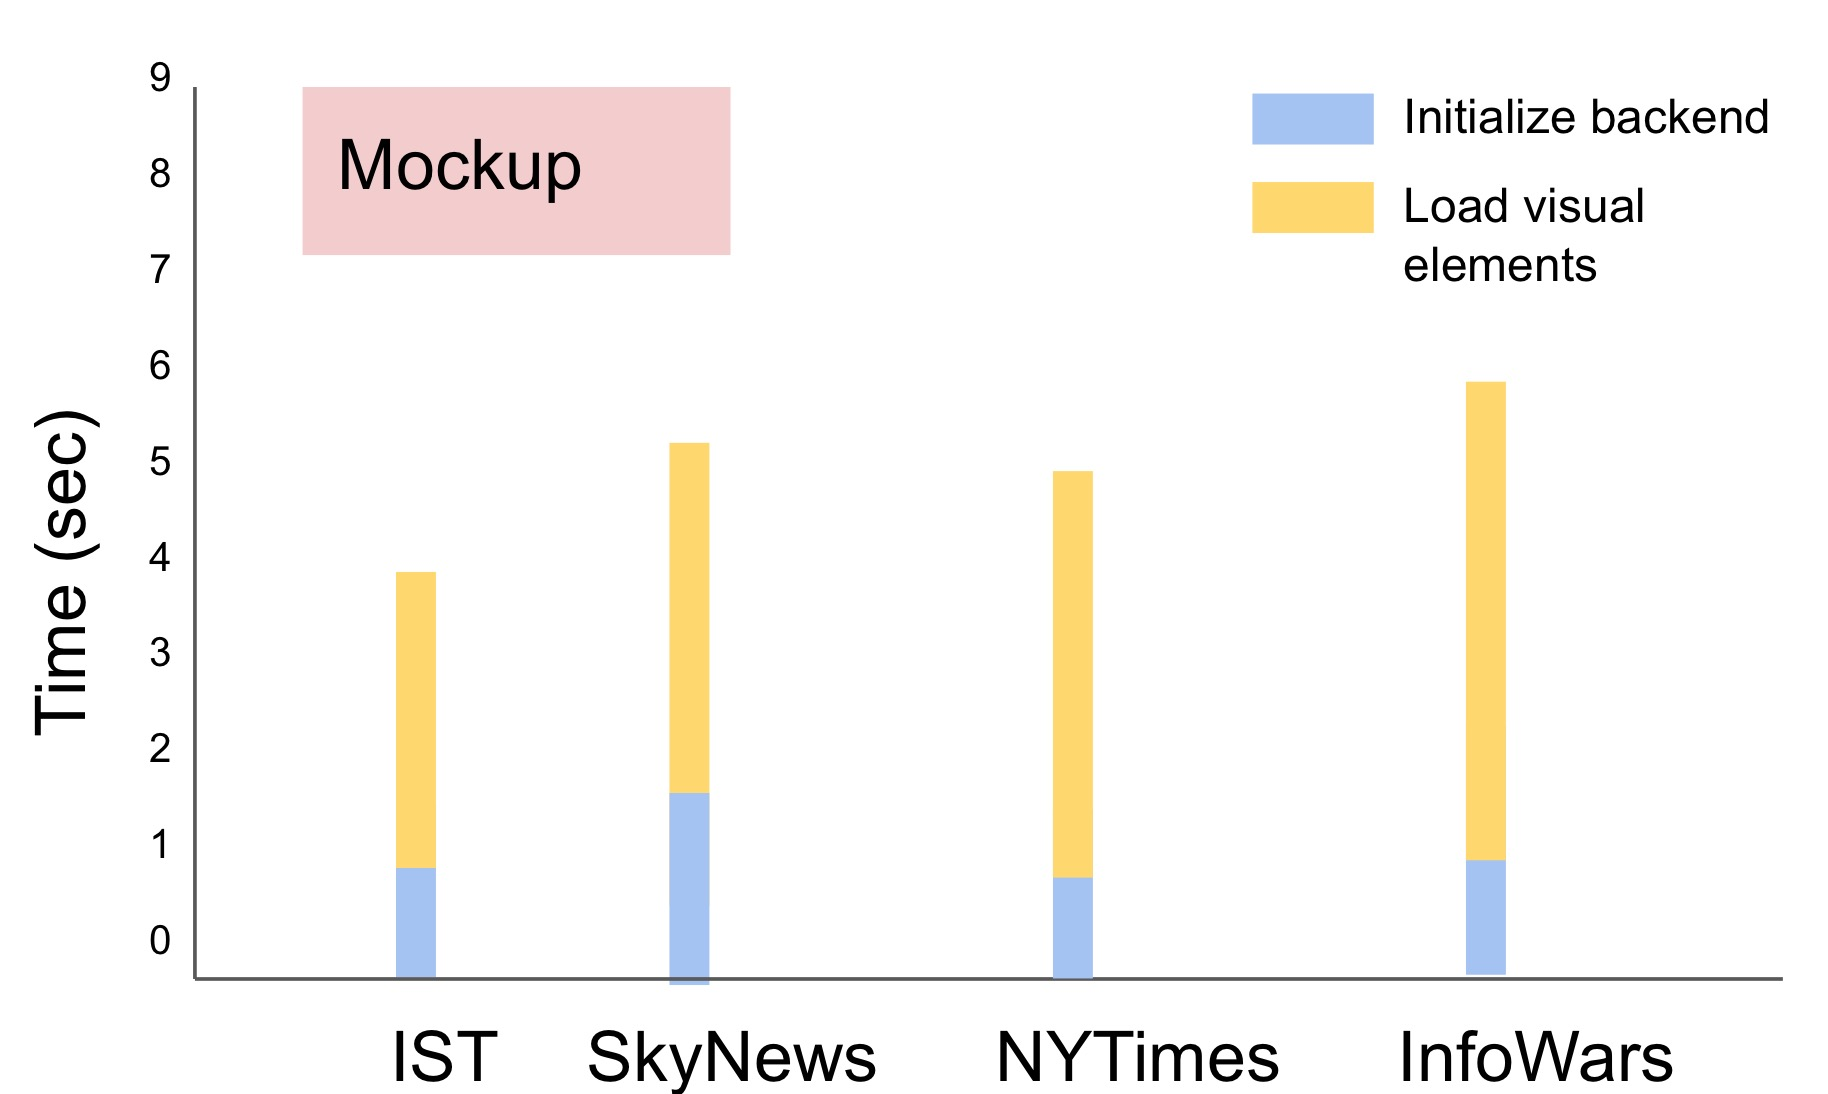
\includegraphics[width=\columnwidth]{mock-figures/timessubcomponents.jpg}
  \vspace{-10pt}
  \caption{Time of drawing the elements and initializing the backend.}
%  \vspace{-0.3cm}
  \label{fig:evalpartial}
\end{figure}

\mypara{2. What is the source of the overheads introduced by DClaims?} Figure~\ref{fig:evalpartial} shows the contributions of two main parts: element drawing and interaction with the backend. \note{NS: @João please change the graph to a compound graph.}
 \note{JS: Didn't have the time to do this one yet}


\begin{figure}[t]
  \centering
  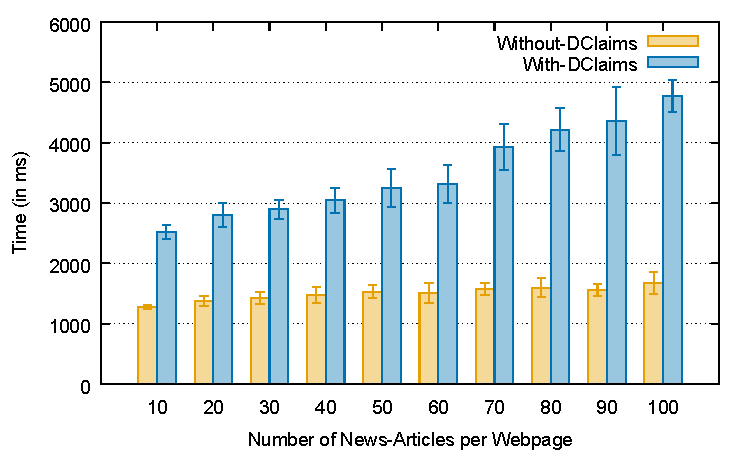
\includegraphics[width=\columnwidth]{final-figures/website-benchmark.pdf}
  \vspace{-10pt}
  \caption{Time to load a webpage as function of the number of articles.}
%  \vspace{-0.3cm}
  \label{fig:evalnarticles}
\end{figure}


\mypara{3. What is the website loading time based on the number of articles in the page?} Figure~\ref{fig:evalnarticles} shows the graph.

\note{JS: I believe this question is answered in the first question " What's the overhead of loading a web page with DClaims?"}

\if0
\begin{figure}[t]
  \centering
  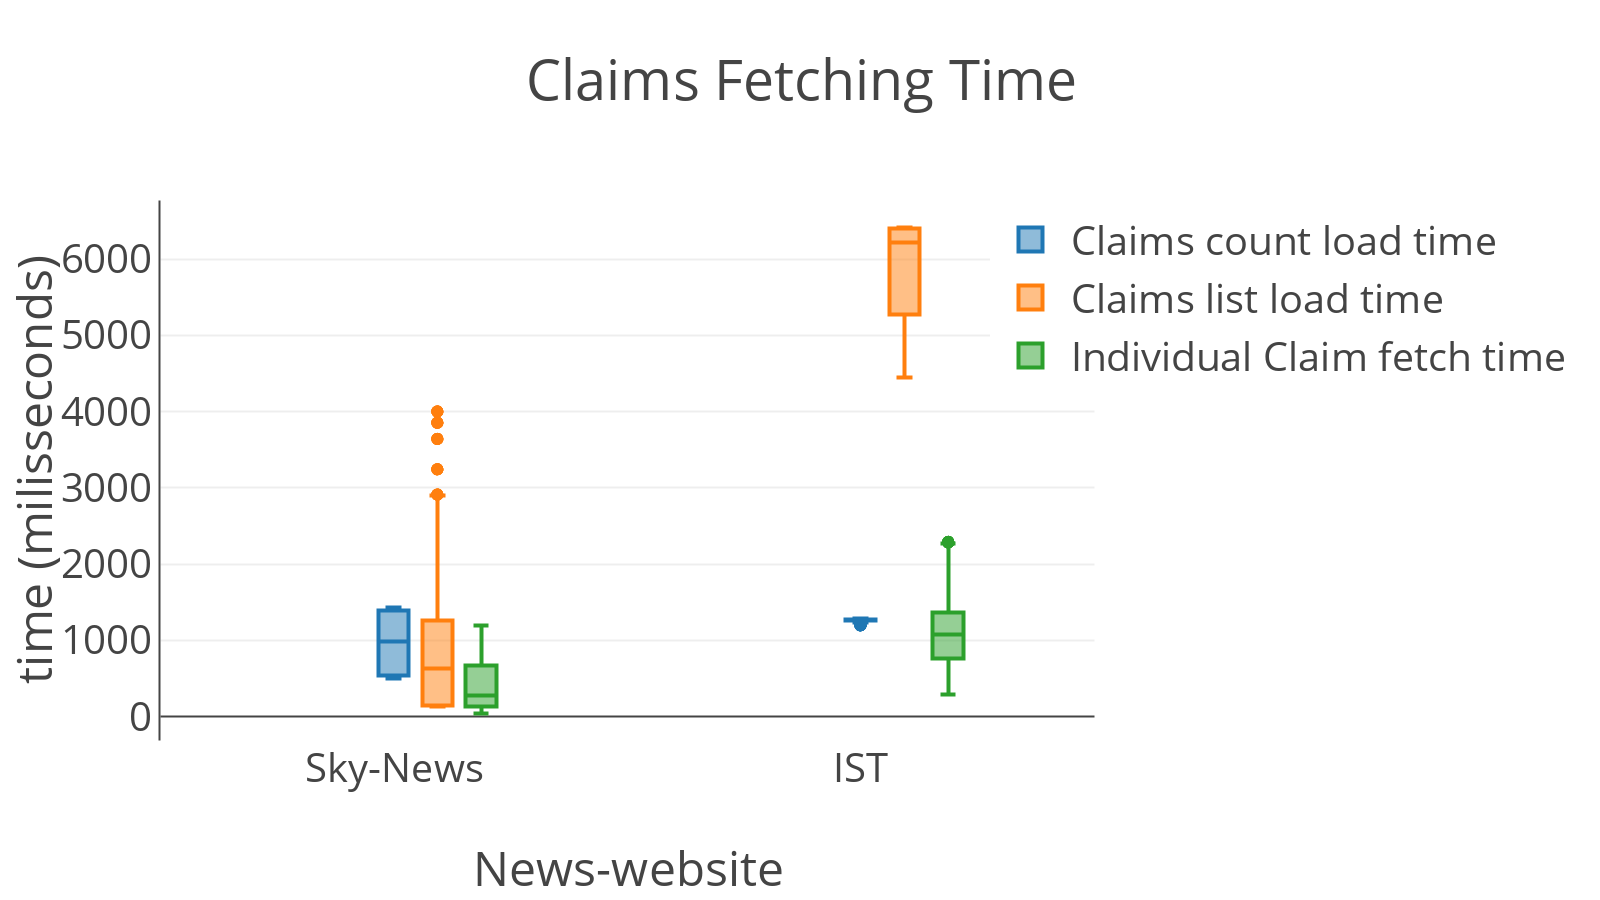
\includegraphics[width=\columnwidth]{figures/chart-fetch.png}
  \vspace{-10pt}
  \caption{Time to retrieve claims on browser.}
%  \vspace{-0.3cm}
  \label{fig:evalclaims}
\end{figure}

\mypara{4. How much time it takes to retrieve the claims of a given article?}
Figure~\ref{fig:evalclaims} shows the time it takes to load a webpage as the number of articles increases. Two curves show the time with and without DClaims.
\fi

\subsection{Performance of the Backend}

We want to evaluate the performance of the backend with respect to the time it takes to retrieve claims.




\mypara{1. What is the claim retrieval time as a function of the number of IPFS nodes in the network?}

Figure \ref{fig:ipfsfetch} shows the time it takes to retrieve individual claims from IPFS. In this experiment we had twenty nodes running DClaims, each node made five claims about random news articles (from a poll of twenty) and then fetched claims from random articles, fetching a new article every ten seconds, for 1400 seconds. \note{fix image x axis label, it should be ten seconds per tick rather than seconds}. Over time the time converges to under ten milliseconds. This happens because of IPFS's cache mechanism, where if a node requests a claim that has requested before, it needs not to ask for it again in the network as a copy is available in their node already. Furthermore, if there are multiple nodes who have the same claim that a given node requests, all those nodes can serve the request.
This chart gives us the following useful information: The longest time that 90\% of the nodes waited for a claim was under one second (outliers were removed ).
Queries are made in parallel, so the time to fetch \textit{n} queries would correspond to the time the slowest query would take.



\subsection{Cost}
Figure \ref{fig:costpublishers} shows the cost of issuing claims in the different available issuance models. The first, individually, corresponds to issuing a claim individually upon its creation. It is the most expensive as it corresponds to the cost of a single issuing transaction (see Table \ref{my-label}), the second one corresponds to the issuance cost if the issuer issued all of his claims once a day (as if he was his own publisher), in this case, the cost is ten times lower, as the transaction cost is divided by the number of claims it carries. Finally, the last modal is using a Publisher, which offers the lowest cost as long as the batch size is higher than the number of claims the person makes in a day.

Figure \ref{fig:timepublishers} shows the confirmation time using the three different issuance mechanisms.
\mypara{Q: How do we know the time it takes with publishers?}
We analyzed three popular news organizations facebook pages and calculated the rate of comments the articles they share receive, which is roughly 4.1 comments per minute. Knowing the batch size in advance, in this case we are using 50, we know the time it takes to fill a batch corresponds to the batch size divided by the rate of claims (which we are assuming is the same as facebook comments).


